
\section{Automatic Topic Labeling}
\label{kap:automaticTL}
%Topics are multinomial distributions a set of recurring themes that are discussed in the collection.

%Topics are a set of recurring themes that are discussed in the collection and represent as a multinomial distribution. Often the top words of the distribution is taken to represent

%of topic modeling can be used. Topic models refer to a set of algorithms that discoverthe topics or hidden thematic structure in a collection of documents. A topic modeltakes a set of documents as the input and outputs topics, a set of recurring themesthat are discussed in the collection, and the degree to which each document expressthese topics (Blei, 2012b). The results of the topic modeling algorithms can be usedto organize, visualize, summarize, and understand large collections of documents.

%A topic is commonly understood to be a a phrase or subject that best describesthe content of a text. In contrast, in topic modeling, every topic is a probabilitydistribution over all words in the collection of documents. In each topic a differentset of words has a high probability and we visualize the topic by listing the mostprobable terms.

Topic Models are used to discover latent topics in a corpus to help to understand large collections of documents. These topics are multinomial distributions over all words in a corpus. Normally, the top terms of the distribution are taken to represent a topic, but these words are often not helpful to interpret the coherent meaning of the topic. Especially, if the person is not familiar with the source collection. For example, for the topic \textit{price, \$, cost, foods, store, product, brand, low, supermarket, good} a  suitable label is \textit{food prices}.\\

With the help of Automatic Topic Labeling (\ac{ATL}) we want to reduce the cognitive overhead of interpreting these topics and, therefore, facilitate the interpretation of the topics.
Of course, the topics can be labeled manually by domain experts, but this method is time consuming if there are hundreds of topics. Additionally, the topic labels can be biased towards the users opinion and the results are hard to replicate. \\

%%TODO human turks?
We are working with domain specific data dealing with organic food. To generate meaningful labels we can not make use of human turks because we need domain experts who are proficient in this area. Therefore, we submitted the topics to our domain experts to label them. But only 50 of the generated topics, ranked according to the importance in a corpus, for each dataset were handed in, in order to not burden them, since this process is very time-consuming. The datasets were labeled by three labelers who tried to find a suitable label, which captures the meaning of the topic and is easily understandable. After labeling, the three labels of a topic were compared and a final label was set. If at least two labelers had the same label, this was taken as the final one. If the given labels were not comparable, no label was set at all. \\

%After labeling, for every dataset three labels suitable to each single topic were compared and a final label was set. 
To relieve our domain experts in the following chapter two approaches for \ac{ATL} are described. In Section \ref{sec:intrinsic} an intrinsic method was used, which is only working on texts and topics from our datasets to generate the labels according \cite{Mei2007}. Section \ref{sec:extrinsic} describes an extrinsic approach by using a lexical database for the English language called \textit{Wordnet} to label the topics.
%The domain experts labeled our topics. There were three labelers who tried to find a suitable label, which captures the meaning of the topic and is easily understandable. After labeling every dataset the three labels were compared and a final label was set. If at least two labelers had the same label, this was taken as the final one. If the given labels were not comparable, no label was set at all.\\


\subsection{Related work}                                                
\label{sec:relWorl: atl}
\textit{\cite{Lau2011}} generated a label set,called primary candidate labels, out of article titles, which were found in Wikipedia or Google by searching the top N words from topics. Afterwards, these labels were chunkized and n-grams were generated. Theses secondary candidate labels were then filtered with the \textit{related article conceptual overlap} (RACO), that removed all outlier labels, such as stop words. Then the primary and secondary candidate labels were ranked by features such as \ac{PMI}, used for measuring association, and the student’s t test. The results were measured with the mean absolute error score for each label, which is an average of the absolute difference between an annotator’s rating and the average rating of a label, summed across all labels. The score lay between 0.5 and 0.56 on a scale from 0 to infinity.

On topics from Twitter \textit{\cite{Zhao2011}} used  a topic context sensitive Page Rank to find keywords by boosting the high relevant words to each topic. These keywords were taken to find keyword combinations (key phrases) that occur frequently in the text collection. The key phrases were ranked according to their relevance,i.e. whether they are related to the given topic and discriminative, and interestingness, the re-tweeting behavior in Twitter. To evaluate the keywords Cohen’s Kappa was used to calculate the iterrater reliability between manually and automatically generated key phrases. The Cohen’s Kappa coefficient was in the range from 0.45 to 0.80, showing good agreement.

\textit{\cite{Allahyari2015}} created a topic model OntoLDA which incorporates an ontology into the topic model and provides \ac{ATL} too. In comparison with \ac{LDA}, OntoLDA has an additional latent variable, called concept, between topics and words. So each document is a multinational distribution over topics, each topic is a multinomial distribution over concepts and each concept is a multinomial distribution over words.  Based on the semantics of the concepts and the ontological relationships among them the labels for the topics are generated in followin steps:
\begin{enumerate}
	\item construction of the semantic graph from top concepts in the given topic
	\item selection and analysis of the thematic graph (subgraph form the semantic graph)
	\item topic graph extraction from the thematic graph concepts
	\item computation of the semantic similarity between topic and the candidate labels of the topic label graph
\end{enumerate}
The top N labels were compared with the labeling from \textit{\cite{Mei2007}} by calculating the precision after categorizing the labels into good and unrelated. The more labels were generated for a topic the more imprecise they got but the preciser \textit{\cite{Mei2007}} labels were.

\textit{\cite{Hulpus2013}} made use of the structured data from DBpedia, that contains structured information from Wikipedia. For each word of the topic the Word-sense disambiguation (WSD) chose the correct sense for the word from a set of different possible senses. Then a topic graph was obtained form DBpedia consisting of the closest neighbors and the links between the correct senses. Assuming the topic senses which are related, lie close to each other, different centrality measures were used and evaluated manually to identify the topic labels. The final labels then were compared to textual based approaches and the precision after categorizing the labels into good and unrelated was calculated.

\cite{Kou2015} captured the correlations between a topic and a label by calculating the cosine similarity between pairs of topic vectors and candidate label vectors. Continuous bag of words (CBOW), Skip-gram and Letter Trigram Vectors were used. The candidate labels were extracted from Wikipedia articles that contained at least two of the top N topic words. The resulting labels for the different vector spaces were compared to automatically generated gold standard labels, representing the most frequent chunks of suitable document titles for a topic. The final labels were ranked by human annotators,too, and were considered as a better solution than the first word of the top N topic words. 

%For topics and preprocessed Wikipedia titles \textit{\cite{Bhatia2016}} used word and title embeddings for both, generated by either doc2vec(for fine-grained labels) or word2vec (for generic labels), to generate topic labels.
%The relevance of each title embedding was measured with the pairwise cosine similarity of the word embeddings for the top N topic words. The sum of of the relevance of doc2vec and vec2doc served as ranking for the labels. The results were evaluated the same way like in \cite{Lau2011}.

For topics and preprocessed Wikipedia titles \textit{\cite{Bhatia2016}} used word and title embeddings. To generate title embeddings doc2vec and word2vec were used to obtain fine-grained labels (doc2vec) or generic labels (word2vec). Given a topic, the relevance of each title embedding was measured based on the pairwise cosine similarity with each of the word embeddings for the top-10 topic terms. The sum of of the relevance of doc2vec and vec2doc served as ranking for the labels. The results were evaluated the same way as like in \cite{Lau2011}.

\textit{\cite{Magatti2009}} used a given tree-structured hierarchy from the Google Directory to generate candidate labels for the topics. These were compared to the topic words by applying different similarity measures. The most suitable label was then selected by exploiting a set of labeling
rules. This approach is applicable to any topic hierarchy summarized by a tree.

\textit{\cite{Mei2007}} generated labels based on the texts collection and their related topics by chunking and building n-grams. They approximated the distribution for the labels and compared these to the distribution of the topic by calculating the \ac{KL} divergence. To maximize the mutual information between the label and the topic distributions the calculated divergence has to be minimized. Three human assessors measured the results and found out that the final labels are effective and robust although applied on different genres of text collections. 


\subsection{Intrinsic Topic Labeling}
\label{sec:intrinsic}
The intrinsic topic labeling is based only on a text collection and therefrom extracted topics.It does not use any external ontologies or embeddings. Because \textit{\cite{Mei2007}} were the only ones who generated topic labels by using an intrinsic approach, we decided to apply their \ac{ATL} on our data, using an implementation from Github\footnote{https://github.com/xiaohan2012/chowmein}. The implementation was adapted to our data and instead of using their preprocessing ours was used.
%TODO: wo sollen die änderungen der implementierung aufgeführt werden?hier?passt das so? ANTWORT: Würdest du die Änderungen noch ausführlicher beschreiben? Was für Änderungen wurden alles vorgenommen? Wenn es so bleibt wie das hier dann passt es. Wenn es umfangreicher wird, solltest du einen seperaten Abschnitt verfassen

In their paper \textit{\cite{Mei2007}} consider noun phrases and n-grams as candidate labels and use \ac{POS}-tags to extract the labels according to some grammar from the text collection. We apply the n-grams approach to select (NN - NN) or (JJ - NN) English and (NN -NN) or (ADJD - NN) German bi-grams as suitable labels for the topics.

The candidate labels were ranked by their semantic similarity to the topic distribution $\theta$. To measure the semantic relevance between a topic and a label \textit{l} a distribution of words \textit{w} for the label $p(w|l)$ was approximated by including a text collection \textit{C} and a distribution $p(w|l,C)$ was estimated, to substitute $p(w|l)$. Then the \ac{KL} divergence $D(\theta||l)$ was applied to calculate the closeness between the label and the topic distribution $p(w|\theta)$. So the \ac{KL} divergence served to capture how well the label fits to the topic. If the two distributions perfectly match each other and the divergence is zero we have found the best label. 
The relevance scoring function of \textit{l}  to $\theta$ is defined as the negative \ac{KL} divergence $-D(\theta||l)$ of $p(w|\theta)$ and $p(w|l)$ and can be rewritten as follows by including \textit{C}:
\begin{align}
\begin{split}
	Score(l,\theta) = &-D(\theta||l) =
	-\sum_{w} p(w|\theta)log\frac{p(w|\theta)}{p(w|l)}\\ =
	&-\sum_{w} p(w|\theta)log\frac{p(w|C)}{p(w|l,C)} -\sum_{w} p(w|\theta)log\frac{p(w|\theta)}{p(w|l)}\\ &-\sum_{w} p(w|\theta)log\frac{p(w|l,C)}{p(w|l)} \\ =
	&-\sum_{w} p(w|\theta)log\frac{p(w,l|C)}{p(w|C) p(l|C)} -D(\theta||C)\\ &-\sum_{w} p(w|\theta)log\frac{p(w|l,C)}{p(w|l)}\\  =
	&-\sum_{w} p(w|\theta) PMI(w,l|C)-D(\theta||C) + Bias(l|C) 
\end{split}
\end{align}
We can see that the relevance scoring function consists of three parts. The first part represents the expectation of \ac{PMI} $E_{\theta}(PMI(w,l|C))$ between \textit{l} and the words in the topic model given the context \textit{C}, the second part is represented by the \ac{KL} divergence between $\theta$ and \textit{C} and the third part can be viewed as a bias using context
\textit{C} to infer the semantic relevance \textit{l} and $\theta$. This bias can be neglected for our data because we have used the same text collection for  producing the topics and the labels. The same applies to the second part, because the \ac{KL} divergence has the same value for all candidate labels. Therefore, we rank the topic labels with 
\begin{equation}
Score(l,\theta) = E_{\theta}(PMI(w,l|C))
\label{Mei:Scoring}
\end{equation}

\begin{figure}[t]
	\begin{minipage}[t]{0.5\textwidth}
		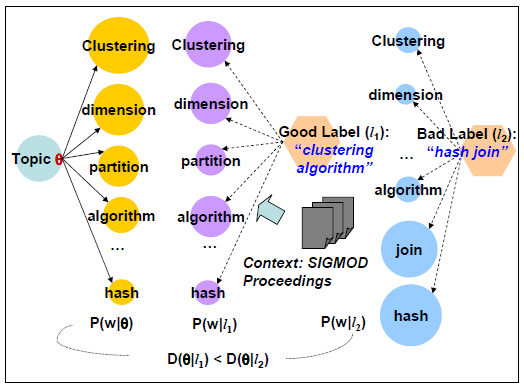
\includegraphics[width=\textwidth]{gfx/Mei/MeiGoodLabel.png}
	\end{minipage}
	\begin{minipage}[t]{0.512\textwidth}
		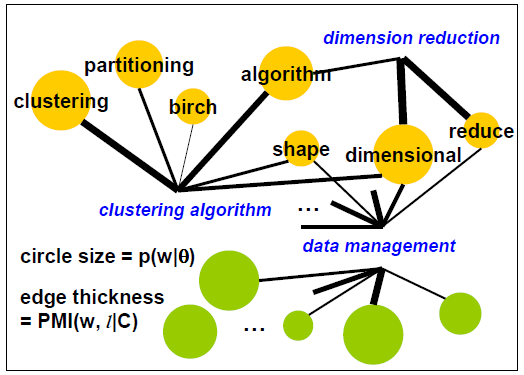
\includegraphics[width=\textwidth]{gfx/Mei/MeiScoring.png}
	\end{minipage}
	\caption[Relevance scoring function for \ac{ATL}]{Relevance scoring function for \ac{ATL}. Adapted from \cite{Mei2007}}
	\label{pic:ScoringFunction}
\end{figure}

The relevance scoring function is also described visually in Figure \ref{pic:ScoringFunction}. The circles represent the probability of terms. The larger the circle the higher is the probability. On the left one can see that the label with lower \ac{KL} divergence is the best one. To approximate $p(w|l)$ in this example the \textit{SIGMOD Proceedings} were used as the text collection \textit{C}, not in our implementation. Analogously, we used our datasets. On the right one can see a weighted graph, where each node is a term in the topic distribution $\theta$ and the edges between terms and the label are weighted by their \ac{PMI}. The weight of the node indicates the importance of a term to the topic, while the weight of each edge indicates the semantical strength between label and term. The relevance scoring function ranks a node higher if the label has a strong semantic relation to the important topical words. Visually, this can be understood that the label is ranked higher if it connects to large circle by a thick edge.

So far only the labeling of a topic was considered, but a characteristic of a good label is the discrimination towards other topics in the topic model, too. It is not useful if many topics have the same labels, although it may be a good label for the topic individually, because we can not make differentiations between the topics. The label should have a high semantic relevance to a topic and low relevance to other topics. In order to take this property into account the $Score(l,\theta)$ in \ref{Mei:Scoring} was adjusted to: 
\begin{equation}
Score'(l,\theta_{i}) = Score(l,\\theta_{i}) - \mu Score(l,\theta_{1,...,i-1,i+1,...})
%Score(l,\theta) = (1+\dfrac{\mu}{k-1}) E_{\theta_{i}}(PMI(w,l|C)) - \dfrac{\mu}{k-1} \sum_{j=1...k} %E_{\theta_{j}}(PMI(w,l|C))
\end{equation}
$\theta_{1,...,i-1,i+1,...}$ describes all topics except the $\theta_{i}$ and $\mu$ controls the discriminative power. In our implementation we set $\mu$ to 0.7.

%The semantic relevance function already guarantees that the label covers the maximal semantic information of $\theta$. Even though one label covers only a topic partially. So a selection of multiple labels for a topic shall cover different aspects of the topic. This is called the intra-topic coverage. For the selection of labels the Maximal Marginal Relevance (MMR) (\cite{Carbonell1998}) was used to get high relevant and low redundant labels.

\subsection{Extrinsic Labeling}
\label{sec:extrinsic}
The majority of literature uses extrinsic topic labeling approaches, using external ontologies or data, because the achieved results are better than the ones from the intrinsic approach. Existing approaches working with e.g. Wikipedia, DBpedia and Google directory as used by \textit{\cite{Lau2011}}, \textit{\cite{Hulpus2013}}, \textit{\cite{Bhatia2016}} and \textit{\cite{Magatti2009}} are not applicable on our specific data. Therefore, we were looking for a method that can be applied on our domain-specific data.

We used the English online database \textit{WordNet}\footnote{http://wordnetweb.princeton.edu/perl/webwn}, that contains 118.000 different word forms and 90.000 word senses. WordNet organizes the several types of words like nouns, verbs, adjectives and adverbs into sets of synonyms, called \textit{synsets}. A \textit{synonym} is a word that has the same meaning as another word. E.g \textit{shut} is a synonym for \textit{close}. These two words form together with possibly other words such as \textit{fold} a synset.
%A synset is a group of words, that have the same meaning for a given word. E.g close, shut and fold represents a synset for the  word close.
Additionally, a synset contains a short definition, called \textit{gloss}, and an exemplary sentence for each term in a synset, which describes the usage of this term. Every distinct word sense of a given word is represented as a separate synset. So the number of different meanings for a word corresponds to the number of synsets. All synsets are linked to each other according to semantic relations such as synonymy, antonymy, hyponymy, hepernymy, meronymy and troponymy. A definition of these semantic relationships can be found in \cite{Miller1995}. In our implementation we used besides \textit{synonymy} also \textit{hypernymy}. If two words can be generalized by an other word, this word is called \textit{hypernym}. E.g \textit{animal} is a hypernym for \textit{cat} and \textit{dog}.

In Figure \ref{pic:Wordnet} one can see the resulting synsets when typing the word \textit{farming} into WordNet. Synsets of nouns (\textit{farming, agriculture, husbandry} and \textit{farming, land}), verbs (two different meanings of \textit{farm} and \textit{grow, raise, farm, produce}) and adjectives (\textit{agrarian, agricultural,farm}) were found, that can be seen on the left side. For each synset the inherited hypernym can be determined. An excerpt of inherited hypernyms(\textit{cultivation,production, industry etc.}) for the synset \textit{farming, agriculture,husbandry} is shown on the right. These are forming a hierarchical tree. The lower a hypernym in the tree the more general it is. In this figure the synset \textit{production} is more general than synset \textit{cultivation}. The most general or lower hypernym for all synsets in WordNet is \textit{entity}. 
\begin{figure}
	\begin{minipage}{0.5\textwidth}
		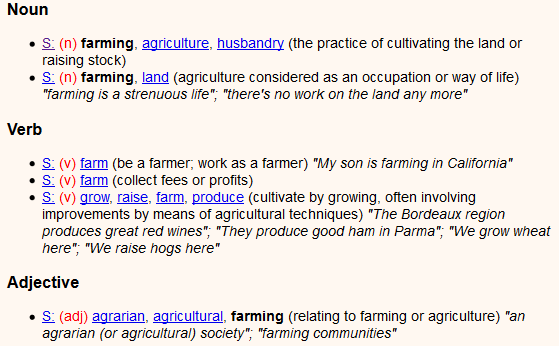
\includegraphics[width=\textwidth]{gfx/Wordnet/farming.png}
	\end{minipage}
	\begin{minipage}{0.5\textwidth}
		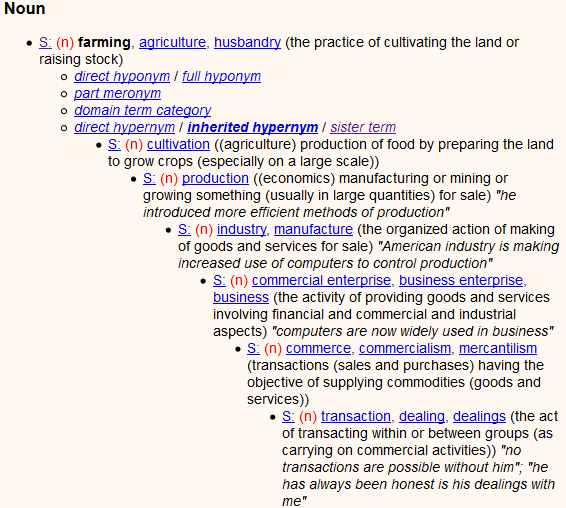
\includegraphics[width=\textwidth]{gfx/Wordnet/farmingTree.png}
	\end{minipage}
	\caption[WordNet results for the word \textit{farming}]{WordNet results for the word \textit{farming}. Adapted from \textit{WordNet}}
	\label{pic:Wordnet}
\end{figure}

To extract the information from WordNet we used the \textit{NLTK corpus reader}.\footnote{http://www.nltk.org/howto/wordnet.html} In addition to WordNet also Polyglot \footnote{https://polyglot.readthedocs.io/en/latest/Embeddings.html} was used as kind of preprocessing for selecting similar words of a topic by using word embeddings.
\subsubsection{Preprocessing}
For all following approaches in the next section we implemented a preprocessing step, that can be applied before running the different approaches for labeling a topic. It should improve the quality of the labels. 
Our topics consists of 10 words, usually these words can not be summarized to one label, which fits to all of the topic words. Therefore, the distances between every combination of two topic words were calculated with Polyglot embeddings. The top-5 words with the lowest distance between each other were selected. On these top words the labeling methods were applied.

\subsubsection{Finding labels with a scoring function}
Trying to find a good label for topics we used topic words \textit{w} and generated synsets \textit{s} for each topic word with the help of WordNet. Based on them we picked their direct hypernyms \textit{h}. To weight the hypernyms \ac{csf} was defined, which includes the number of hypernyms \textit{h} for the word \textit{w} and the number of words, that have a hypernym in common. When a hypernym for a word was found the reciprocal of the total number of hypernyms for each word was assigned to to every hypernym of the current word. If a selected hypernym is used by another word, too, the scores are added and then multiplied by the number of common words. We select the final label by the highest score.

Figure \ref{pic:HypFun} illustrates the scores for each hypernym, which are represented as circles above the hypernyms. The arrows connect the topic words \textit{w} with their synsets \textit{s}. These are connected to hypernyms \textit{h}. For $w_{1}$ each hypernym $h_{1},h_{2}$ has the value $\tfrac{1}{3}$. {$h_{4}$ and $h_{5}$ have the value $\tfrac{1}{2}$, 
	but $h_{5}$ is connected to $s_{5}$ and $s_{6}$. Therefore, we add up $\tfrac{1}{2}$ from $w_{2}$ and $\tfrac{1}{3}$ from $w_{3}$ and multiply the result by 2. In total $h_{5}$ reaches the highest score of $\tfrac{5}{3}$ and is selected as the final label.

\begin{figure}
	\centering
	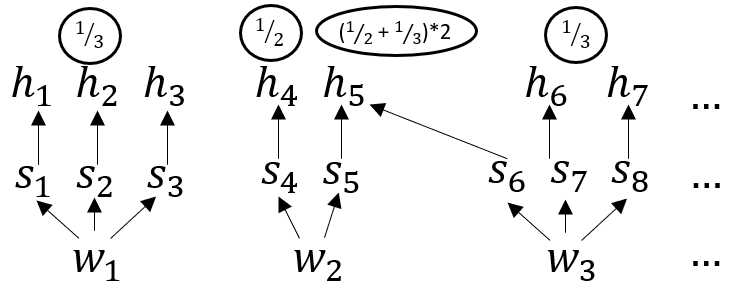
\includegraphics[width=0.5\textwidth]{gfx/Wordnet/HypFunF.png}
	\caption[\ac{ATL}: Scoring function for hypernyms]{Scoring function for hypernyms}
	\label{pic:HypFun}	
\end{figure}

\subsubsection{Find labels with similarity functions}
The first one utilizes similarity functions provided by WordNet. The second one relies on Polyglot word embeddings to calculate the distance between two terms.

%TODO:verb und nomen vgl nicht möglich, erwähnen? ANTWORT: Ich denke das ist nicht notwending. Das macht die Erklärung nur verwirrender. Auf Nachfrage kannst du das bei der Präsentation genauer erklären
WordNet offers different similarity functions, to calculate the similarity between synsets:
\begin{itemize}
\item The \textit{path-similarity} is defined by the nodes, which are visited while going from one word to another using the hypernym hierarchy. The distance between two words is the number of nodes that lie on the shortest path between two words in the hierarchy. The calculated score is in range of 0 and 1, while 1 means two words are identical.
\item The \textit{lch-similarity} (Leacock-Chodorow) is based on the shortest path $p$ and the maximum depth $d$ of the hierarchy in which the words occur. The path length is scaled by the maximum depth: $-log(p/2d)$\newline
\end{itemize}
The remaining three similarity functions are measuring the \ac{IC} of synsets. \ac{IC} combines the knowledge of the hierarchical structure from WordNet, with statistics on actual usage in text as derived from a large corpus. Per default WordNet uses the Brown Corpus. Although, this corpus is not related to our domain-specific data, it includes a large number of English texts and is suitable as a reference corpus for this specific task. 

\begin{itemize}
\item The \textit{res-similarity} (Resnik-Similarity) weights edges between nodes by their frequency of the used textual corpus. Based on the \ac{IC} of the Least Common Subsumer (lsc), the most specific ancestor node, a similarity score is calculated.
\item The \textit{jcn-similarity}(Jiang-Conrath Similarity) calculates the relationship between two words with $(IC(w_{1}) + IC(w_{2}) - 2 * IC(lcs))$ and \item the \textit{lin-similarity} calculates it with $2 * IC(lcs) / (IC(w_{1}) + IC(w_{2}))$.
\end{itemize}
%path sim better then ich because the labels were more specific.
% bsp mit tabelle, wie oft entity, abstraction, physical entity,physical object,whole
%und beispiel mit 3topics, dass die labels besser sind

For all topic words we generated synsets and calculated for all possible combinations of the topic words the similarities of their synsets. For every possible topic word pair the highest similarity score from the synsets was taken and the lowest common hypernym was derived. If a combination of topic words had the same lowest common hypernym, the similarities were summed up. In the end, the hypernym with the highest score was taken as the final label. 

The same procedure was applied also with Polyglot embeddings (plg). Instead of calculating the similarity between the synsets with WordNet similarity functions, the distance function from the Polyglot library was used. The lower the distance between two words the more similar they are. The other steps remained the same.

\subsection{Evaluation}
%TODO im anhang nur wortvertilungen kein topic vergleich, ist das ok, fur alle daten. Oder auch topics zum veranschaulichen rausziehn? Oder komplett bleiben lassen und nur die english editrial nehmen? ANTWORT: Zunächst bleiben lassen wenn zum Schluss Zeit über ist, kannst du den Anhang noch um die anderen Datasets erweitern. Wenn du das machst, reicht es die Wortverteilungen zu plotten.
In the following section the results of intrinsic and extrinsic topic labeling will be evaluated regarding their quality and the number of different labels in a topic model. The labels generated automatically, are also compared to the manual labels, assigned by the domain experts. For evaluation we used English editorial articles.%TODO hier erwähnen? ANTWORT: Was willst du hier erwähnen? das wir nur english editorials im text behandeln
%In section \ref{eval:intrinsic} we evaluate the intrinsic and in section \ref{eval:extrinsic} the extrinsic topic labeling. Afterwards, the the intrinsic and extrinsic labellings are compared with each other in section \ref{eval:comparison}. 
First, we evaluate the intrinsic and second, the extrinsic topic labeling. Afterwards, the the intrinsic and extrinsic labellings are compared with each other. 

\subsubsection{Intrinsic topic labeling}
\label{eval:intrinsic}
We applied the \ac{ATL} in section \ref{sec:intrinsic} on our Dataset, which include editorials, comments and forums. In general, the \ac{ATL} according to \cite{Mei2007}, outputs only different labels for topics, which were generated with \ac{LDA}. For the topics generated with \ac{NMF} the same label was given for every topic in a topic model. The reason could be, that \ac{NMF} does not have a probability distribution for $\theta$, but although we normalized it to numbers between 0 and 1, it was not helpful. Therefore, the labels for topics generated with \ac{NMF} were neglected. Further evaluations are based on English editorial articles. 
\paragraph{Topics from Generation 1}
First, we used the topics from \textit{Generation 1}, which were generated by using collocations as described in \ref{data:preprocessing}. In Figure \ref{fig:labelcount_intrinsic} the label counts for English editorial articles are shown. On the x-axis all labels are listen while the y-axis denotes the number of same labels. 
Considering the labels without a concrete topic assignment one can see, that they are meaningful and specific. Often, a label is a persons name e.g {\textit{Jose Andres, Rahm Emanuel, Morgan Stanly,Gloria Casas, Theresa Eisemann etc.}}.
%mai with2bigrams
\begin{figure}[h]
	\centering
	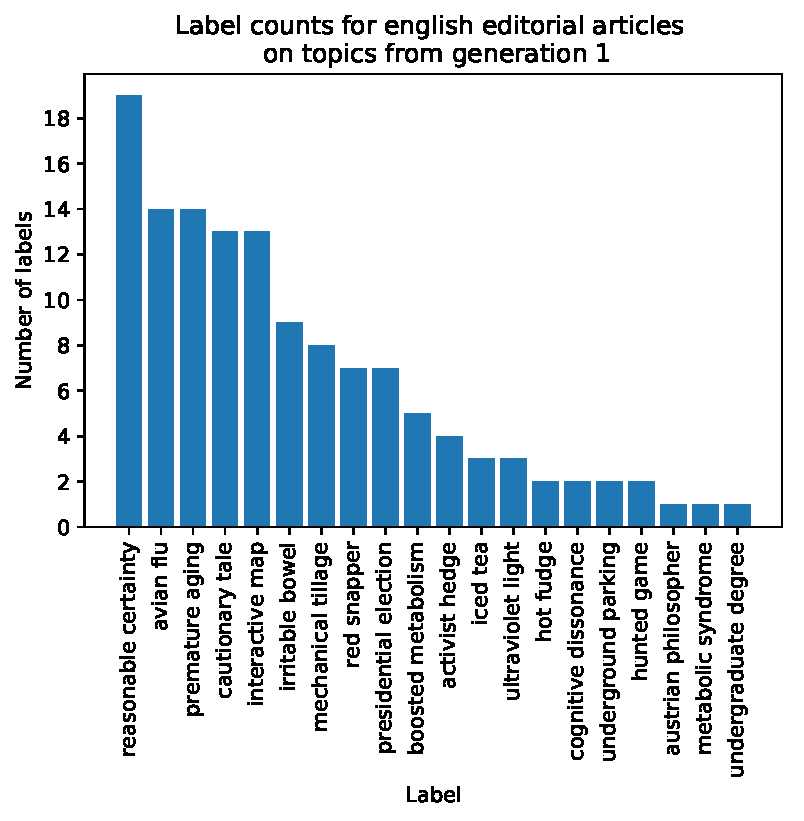
\includegraphics[width=7cm]{gfx/POS-gen1/alte_topics.pdf}
	\caption[Label counts for topics from Generation 1 with intrinsic labeling]{Label counts for topics from Generation 1 according to \cite{Mei2007}.}
	\label{fig:labelcount_intrinsic}
\end{figure}

In Table \ref{tab:extrinsic_manually} example topics are shown, which were labeled manually by domain experts and with the intrinsic approach. The intrinsic labels do not really fit to the given topic: \textit{Rahm Emanuel} an American politician is assigned to Topic 107, which deals with environment and waste. \textit{Hairy vetch}, a plant variety, for Topic 23. \textit{Irritable bowel syndrome}  to Topic 64 and \textit{Safran Foer}, an American novelist, to Topic 74, dealing with animal husbandry. The automatic labels have nothing in common with the manual ones.
% mai label und hannah
%%tabelle mit hannas
\begin{table}[h]
	\begin{minipage}[t]{0.5\textwidth}
		\begin{tabular}{c|l}
			&Topic 107 \\
			\hline
			method & \thead{waste, compost, use, scrap, material,\\landfill, ton, environmental, throw, gas} \\
			\hline
			intrinsic & rahm emanuel  \\
			manual &waste	\\
			&\\
			%{topic 107}
		\end{tabular}
	\end{minipage}
	\begin{minipage}[t]{0.5\textwidth}
		\begin{tabular}{c|l}
			&Topic 23 \\
			\hline
			&\thead{grow, garden, plant, farm, vegetable, \\seed, year, tomato, produce, farming} \\
			\hline
			&hairy vetch\\
			&homegrown food	\\
			\\
			%{topic 23}
		\end{tabular}
	\end{minipage}
	\begin{minipage}[t]{0.5\textwidth}
		\begin{tabular}{c|l}
			&Topic 64\\
			\hline
			method& {\thead{milk, raw, dairy, product, cheese,claim,\\ health, cow drink, study }} \\
			\hline
			intrinsic &irritable bowel syndrome\\
			manual&dairy product\\
		\end{tabular}
	\end{minipage}
	%{topic 64}
	\begin{minipage}[t]{0.5\textwidth}
		\begin{tabular}{c|l}
			&Topic 74 \\
			\hline
			&\thead{meat, feed, beef, animal, grass,\\cow, eat, raise, buy, make} \\
			\hline
			&safran foer\\
			&animal husbandry	\\
		\end{tabular}
	\end{minipage}
	%{topic 74}
	\caption[Labeled topics manually and with intrinsic method and ]{Topics labeled manually and with intrinsic methods.}
	\label{tab:extrinsic_manually}
\end{table}

\paragraph{Topics including POS-tagging:}
%In their paper \textit{\cite{Mei2007}} consider noun phrases and n-grams as candidate labels and use \ac{POS}-tags to extract the label according to some grammar from the text collection. We apply the n-grams approach to select (NN - NN) or (JJ - NN) English and (NN -NN) or (ADJD - NN) German bi-grams as suitable labels for the topics.
%TODO soll die pos taggs genannt werden, auch wenn ich nur hier englische nehme? ANTWORT: Hinweis dass mit Spacy getagged wurde und in den Fußnoten ein Link zu der Seite die die POS-Tags erklärt

By providing \ac{POS}-tags, using Spacy\footnote{Possible POS-tags: https://spacy.io/api/annotation}, we can limit the canidate labels to certain word types. In our experiments we used (NN-NN) or (JJ-NN) \ac{POS}-tags for English topic labels and (NN-NN) or (ADJD-NN) for German.  To apply \ac{POS}-tagging, the preprocessing for the texts had to be changed, because in Generation 1, a collocation finder was used. After performing this step the \ac{POS}-tags can not be applied retroactively. We removed collocation finding and added \ac{POS}-tagging. All other preprocessing steps remained the same. Nevertheless, the topics differ from the ones of Generation 1. 

In Table \ref{tab:intrinsic_label_pos} topics and labels are shown with different \ac{POS}-tags. In comparison to the labels generated without \ac{POS}-tagging, these labels seem closer to a topic. For Topic 6, 10, 23 and 37 the labels \textit{music festival, premature aging, hunted games} and \textit{modified organism} seem good.

%with pos and without
\begin{table}[h]
	\begin{minipage}[t]{0.5\textwidth}
		\begin{tabular}{c|c}
			&Topic 6\\
			\hline
			with \ac{POS}-tags & \thead{restaurant, fast, chain, meal,\\ say, menu, ingredient,\\ burger, chipotle, mcdonald } \\
			\hline
			(NN, NN) & music festival   \\
			(JJ, NN) & hot fudge \\
			-  & dunkin donuts\\
			&\\
		\end{tabular}
		%{topic 6}
	\end{minipage}
	\begin{minipage}[t]{0.5\textwidth}
		\begin{tabular}{c|c}
			&Topic 10\\
			\hline
			& \thead{child, eat, kid,\\ parent, family,	healthy,\\ school, who, 	health,can } \\
			\hline
			& anorexia nervosa \\
			& premature aging   \\
			& anorexia nervosa	\\
			&\\
		\end{tabular}
		%{topic 10}
	\end{minipage}
	\begin{minipage}[t]{0.5\textwidth}
		\begin{tabular}{c|c}
			&Topic 23\\
			\hline
			with \ac{POS}-tags &  \thead{meat, beef, feed,animal, grass,\\ cattle,eat,\\ raise, more, pork} \\
			\hline
			(NN, NN) & sport utility \\
			(JJ, NN) & hunted game   \\
			-& earl butz	\\
		\end{tabular}
	\end{minipage}
	\hfill\hfill
	%{topic 23}
	\begin{minipage}[t]{0.5\textwidth}
		\begin{tabular}{c|c}
			&Topic 37\\
			\hline

			& \thead{carbon, climate, gas,\\ 	greenhouse, emission, change,\\ 	reduce, 	global, 	industrial, 	co2} \\
			\hline
			& gene splicing  \\
			& interactive map   \\
			& modified organisms\\
		\end{tabular}
	\end{minipage}
	%{topic 37}
	\caption[Labeled topics according with intrinsic method]{Labeled topics with intrinsic method}
	\label{tab:intrinsic_label_pos}
\end{table}

%TODO: besser ausdrücken, dass keine postags angewandt wurden, aber es trotzdem nicht die topics von generation 1 sind. ANTWORT: Ich denke das wird bereits klar. Höchstens in der Bildunterschrift noch erklären. Erklärung im Fließtext ist nicht nötig
In Figure \ref{fig:labelcount_intrinsic_pos} the label counts for English editorial articles using the texts, that were \ac{POS}-tagged are shown. On the x-axis all labels are listen while the y-axis denotes the number of same labels. 
In the plots where \ac{POS}-tags were applied, no labels include a name of persons and a smaller number of labels was outputted in contrast to the plot without \ac{POS}-tags. 

However, the same observation can be made as above. Although, the labels seem meaningful and specific they do not really fit to the topics. We assume that the high quality of the labels themselves stem from the way they are generated. By applying bi-gram mining on the original corpus only useful word combinations are found as candidate labels. That the labels seemingly don’t fit to the topics means that measuring the relatedness between the topics and the labels by their KL-divergence is not successful on our data.

%label counts for pos
\begin{figure}[h]
	\centering
	\begin{minipage}[t]{0.5\textwidth}
		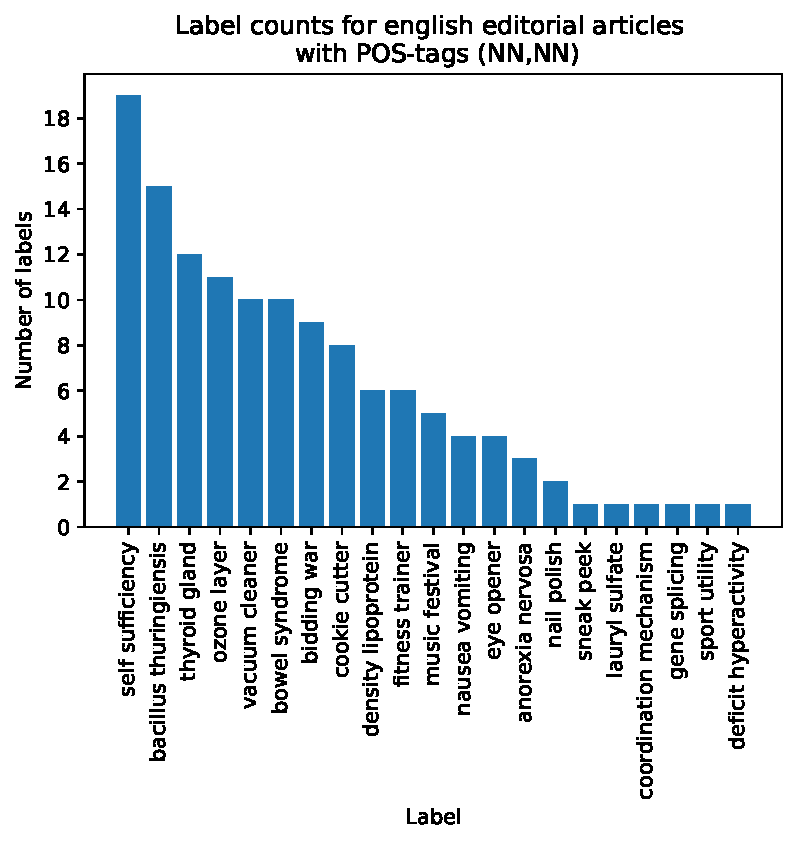
\includegraphics[width=7cm]{gfx/POS-gen1/mit_NN.pdf}
	\end{minipage}%
	\begin{minipage}[t]{0.5\textwidth}
		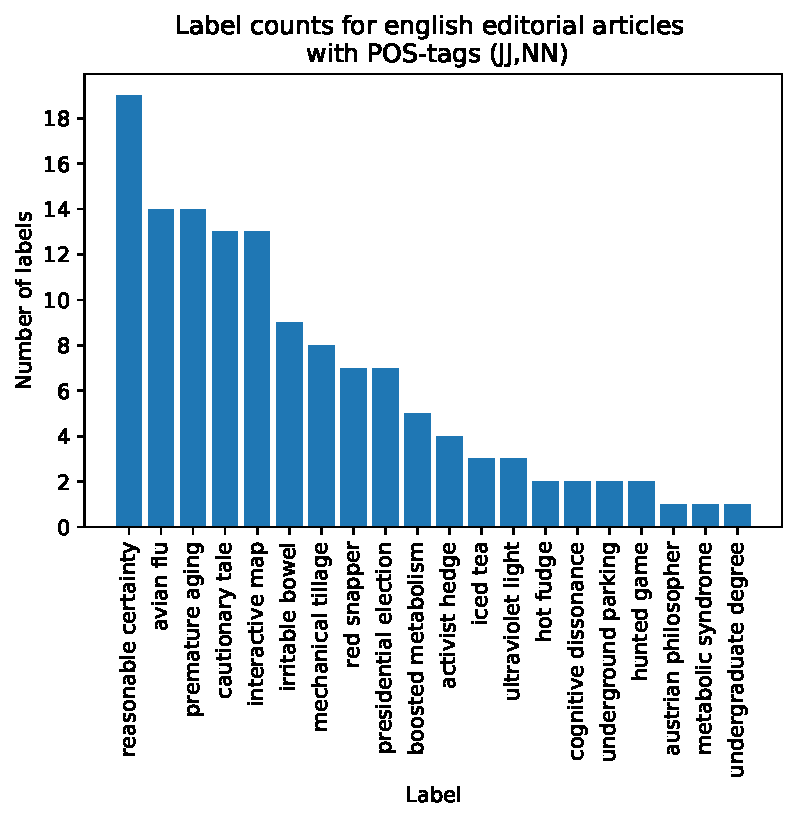
\includegraphics[width=7cm]{gfx/POS-gen1/mit_JJNN.pdf}
	\end{minipage}
	\begin{minipage}[t]{0.5\textwidth}
		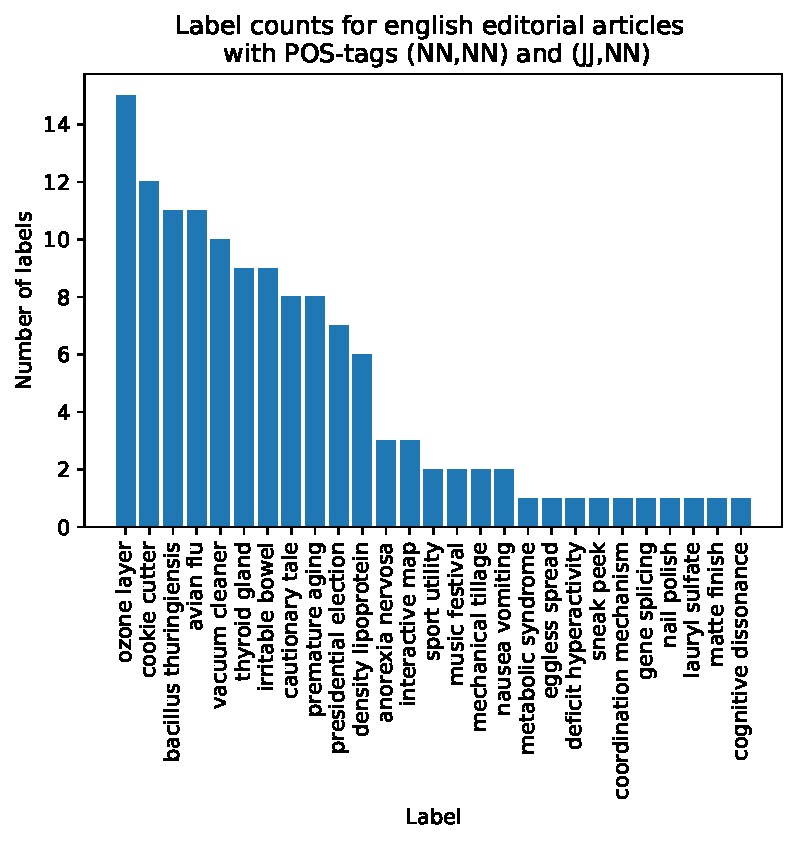
\includegraphics[width=7cm]{gfx/POS-gen1/mit_beiden_pos.pdf}
	\end{minipage}%
	\begin{minipage}[t]{0.5\textwidth}
		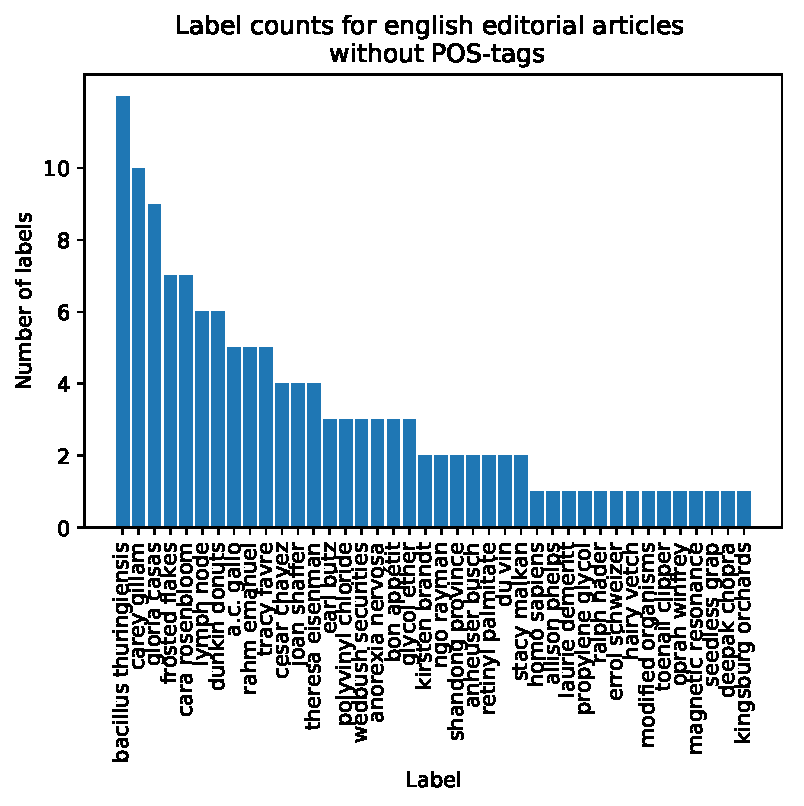
\includegraphics[width=7cm]{gfx/POS-gen1/ohne_POS.pdf}
	\end{minipage}%
	\caption{Label counts for topics including \ac{POS}-tags with intrinsic method.}
	\label{fig:labelcount_intrinsic_pos}
\end{figure}

\subsubsection{Extrinsic topic labeling}
\label{eval:extrinsic}
%TODO keine anhang infos für andere daten... hab alles per hand gemacht...
We applied the \ac{ATL} in section \ref{sec:intrinsic} on our Dataset, using the English online database WordNet and Polyglot embeddings. The different similarity functions from WordNet, the \ac{csf} and the Polyglot embeddings were used to label our topics. A few examples are shown in Table \ref{tab: labeled_extrinsic_and_manually} including the manual assigned labels to the topics, too. Some labels generated with the automatic approaches match with the manual assigned labels. This is the case for the Topics 64, 84 and 107. For the other topics, the labels heading to the right direction as the manual label: for Topic 97 \textit{chemical} and manually \textit{pesticide residues}, for Topic 99 \textit{bee} and manually \textit{beekeeping} and for Topic 109 \textit{grocery store, mercantile establishment, marketplace} and manually \textit{retailers} was assigned.
%%tabelle mit hannas
\begin{table}
	\begin{minipage}[t]{0.5\textwidth}
		\begin{tabular}{c|ll}
			&Topic 23 &\\
			\hline
			method&\multicolumn{2}{l} {\thead{grow, garden, plant, farm, vegetable, \\seed, year, tomato, produce, farming}} \\
			\hline
			path&entity 	& produce  \\
			ich&entity	& produce\\
			res&produce		& produce\\
			jsn&produce	& produce\\
			lin&produce		& produce\\
			plg&vegetable	& vegetable\\
			\ac{csf}&cultivate  & cultivate\\
			manual&\multicolumn{2}{l}{homegrown food}	\\
			&\\
			%{topic 23}	
		\end{tabular}
	\end{minipage}
	\begin{minipage}[t]{0.5\textwidth}
		\begin{tabular}{c|ll}
			&Topic 64 &\\
			\hline
			& \multicolumn{2}{l} {\thead{milk, raw, dairy, product, cheese,  cow\\health, drink, study, claim }} \\
			\hline
			& abstraction 	& beverage  \\
			& abstraction	& produce\\
			& \textbf{dairy product}		& beverage\\
			& produce	& beverage\\
			& beverage		& beverage\\
			& \textbf{dairy product}	& abstraction\\
			& nakedness  & farm\\
			& \multicolumn{2}{l}{\textbf{dairy product}}	\\
			&&\\
			%topic 64
		\end{tabular}
	\end{minipage}
	\begin{minipage}[t]{0.5\textwidth}
		\begin{tabular}{c|ll}
			&Topic 74 &\\
			\hline
			method&\multicolumn{2}{l} {\thead{meat, feed, beef, \\ grass, eat, raise, cow, buy, make, animal}} \\
			\hline
			path&entity 	& meat  \\
			ich&entity	& abstraction\\
			res&matter		& meat\\
			jsn&food	& meat\\
			lin&matter		& meat\\
			plg&cattle	& physical entity\\
			\ac{csf}&cattle  & be\\
			manual&\multicolumn{2}{l}{animal husbandry}	\\
			&&\\
			% {topic74}
		\end{tabular}
	\end{minipage}
	\begin{minipage}[t]{0.5\textwidth}
		\begin{tabular}{c|ll}
			&Topic 84 &\\
			\hline
			& \multicolumn{2}{l} {\thead{company, tea, brand, product, drink, \\honest, new, beverage, consumer, 	goldman}} \\
			\hline
			& \textbf{beverage}  & \textbf{beverage}\\
			& physical entity	& substance\\
			& substance	& substance\\
			& \textbf{beverage}		& \textbf{beverage}\\
			& \textbf{beverage}	& \textbf{beverage}\\
			& food 	& food  \\
			& \textbf{beverage}	& \textbf{beverage}\\
			& \multicolumn{2}{l}{\textbf{beverage}}	\\
			&&\\
			%topic 84
		\end{tabular}
	\end{minipage}
	\begin{minipage}[t]{0.5\textwidth}
		\begin{tabular}{c|ll}
			&Topic 97 &\\
			\hline
			method&\multicolumn{2}{l} {\thead{fruit, vegetable, pesticide, produce, buy, \\eat, list, apple, residue, sweet}} \\
			\hline
			path& matter& matter\\
			ich&matter	& matter\\
			res&matter	& matter\\
			jsn&matter	& matter\\
			lin&produce	& matter\\
			plg&fruit  & entity\\
			\ac{csf}&chemical 	& chemical\\
			manual&\multicolumn{2}{l}{pesticide residues}	\\
			&&\\
			%{topic 97}
		\end{tabular}
	\end{minipage}
	\begin{minipage}[t]{0.5\textwidth}
		\begin{tabular}{c|ll}
			&Topic 99 &\\
			\hline
			& \multicolumn{2}{l} {\thead{bee, honey, study, hive, year, \\beekeeper, plant, researcher, honeybee, colony}} \\
			\hline
			& organism & person  \\
			& organism	& person\\
			& organism	& organism\\
			& organism	& whole\\
			& bee	& artifact\\
			& bee	& artifact\\
			& farmer 	& scientist\\
			& \multicolumn{2}{l}{beekeeping}\\
			&&\\
			%topic 99
		\end{tabular}
	\end{minipage}
	\begin{minipage}[t]{0.5\textwidth}
		\begin{tabular}{c|ll}
			&Topic 107 &\\
			\hline
			method & \multicolumn{2}{l} {\thead{waste, compost, use, scrap, material, \\landfill, ton, environmental, throw, gas}} \\
			\hline
			path & material 	& material  \\
			ich  & abstraction	& physical entity\\
			res  & material		& material\\
			jsn  & abstraction	& material\\
			lin  & material		& material\\
			plg & \textbf{waste}	& abstraction\\
			\ac{csf} & convent  & lowland\\
			manual & \multicolumn{2}{l}{\textbf{waste}}	\\
		\end{tabular}
	\end{minipage}
	\begin{minipage}[t]{0.5\textwidth}
		\begin{tabular}{c|ll}
			&Topic 109 &\\
			\hline
			& \multicolumn{2}{l} {\thead{foods, company, store, chain, market,\\ executive, new, year, mackey,	grocery}} \\
			\hline
			& grocery store 	& mercantile establishment\\
			& physic entity	& mercantile establishment\\
			& social group	& mercantile establishment\\
			& grocery store	& mercantile establishment\\
			& social group	& mercantile establishment\\
			& artifact	& abstraction\\
			& marketplace  & marketplace\\
			& \multicolumn{2}{l}{retailer}	\\
			%topic 84
		\end{tabular}
	\end{minipage}
	%{topic 74}
	\caption[Labeled topics with extrinsic methods and manually]{Topics labeled from Generation 1 manually and with extrinsic methods. Labels including preprocessing are in the third and fifth column. \textbf{Bold} words are the same as the manual assigned label.}
	\label{tab: labeled_extrinsic_and_manually}
\end{table}
Evaluating the automatically generated labels using different approaches, it was discovered that depending on the topics different labeling techniques output the best labels. It is not possible to tell, which approach is the best for all topics, let alone for several topic models according to the labels. Therefore, we tried to evaluate the labels generated with the extrinsic methods according to label counts. The words \textit{entity, physical entity, object, whole, matter} and \textit{abstraction} were chosen, because these are the most general words in the hierarchical tree of hypernyms in WordNet and do not have a high informative value. 
In Table \ref{tab: label_count_non_informative} the number of non informative words are listed for the different similarity functions from WordNet. Based on the sum of the non informative words per similarity function and Polyglot embeddings (plg), we ranked the different methods in Table \ref{tab:ranked_non_info}. The top 3 are: res-similarity with preprocessing, lin-similarity with preprocessing and Polyglot embeddings.
%%labelcount uninformative words
\begin{table}[h]
	\begin{tabular}{c|c|c|c|c|c|c|c}
		%& \multicolumn{6}{c}{Count of labels}\\
		%\hline
		method & entity	& physical entity & object & whole & matter & abstraction & $\sum$ \\
		\hline
		path& 19		&20				  &7	   &4      &1       &33 &84\\
		& \textbf{7}&\textbf{7}	 &\textbf{5}  &\textbf{2} &\textbf{1} &\textbf{16} & 38\\
		\hline
		ich& 29		&23				  &7	   &4      &1       &42 & 106\\
		& \textbf{13}&\textbf{13}	 &\textbf{9}  &\textbf{3} &\textbf{1} &\textbf{25} & 64\\
		\hline
		res& -		&4				  &5	   &4      &9       &5 &27\\
		& -			&\textbf{2}	 &\textbf{4}  &\textbf{1} &\textbf{2} &\textbf{1} &10\\
		\hline
		jsn& 19		&14				  &3	   &2      &1       &25 &64\\
		&10 		&\textbf{6}	 &\textbf{2}  &\textbf{2} &\textbf{2} &\textbf{9} &31\\
		\hline
		lin& -		&1				  &8	   &6      &9       &11 &35\\
		& -	 	&\textbf{1}	 &\textbf{3}  &\textbf{5} &\textbf{3} &\textbf{5} &17\\
		\hline
		plg& 1		&1		 &3	   &6      &4       &3 &18\\
		& \textbf{7}&\textbf{7}	 &\textbf{4}  &\textbf{7} &\textbf{3} &\textbf{19} & 47\\
	\end{tabular}
	\label{tab: label_count_non_informative}
	\caption[Label counts of non informative words]{Label counts of non informative words with different similarity functions. \textbf{Bold} numbers denote labels including preprocessing.}
	%fett sind die preprzesseten labels
\end{table}
\begin{table}[h]
	\begin{tabular}{|l|l|l|}
		\hline
		1. \textbf{res-similarity} &2. \textbf{lin-similarity} &
		3. polyglot embeddings (plg) \\ 
		\hline
		4. res-similarity&5. \textbf{jsn-similarity}& 6. lin-similarity\\
		\hline
		7. \textbf{path-similarity} &8. \textbf{polyglot embeddings} &9. jsn-similarity \\ 
		\hline
		10. \textbf{ich-similarity}&11. path-similarity  &12. ich-similarity\\
		\hline
	\end{tabular}
\caption[Ranked similarity functions for extrinsic labeling]{Ranked similarity functions. \textbf{Bold} similarities denote the similarities, which were applied on preprocessed topics.}
\label{tab:ranked_non_info}
\end{table}
%TODO kling iwie komisch... weglassen? sollte dann eig auch die verteilung für die verschiedenen similarities machen.
The labels with \ac{csf} does not include any non informative words, because the only the direct hypernyms and not the whole hierarchy of hypernyms was considered. Therefore, we plotted the amount of distinct labels in Figure \ref{extr_csf_count}. This shows, the labels generated with preprocessing on the left side and the labels without on the right. The number of same labels is maximal at 6 or 8, which shows that the labels are discriminative.
%TODO label counts noch einbringe?
\begin{figure}[h]
	\begin{minipage}[t]{0.5\textwidth}
		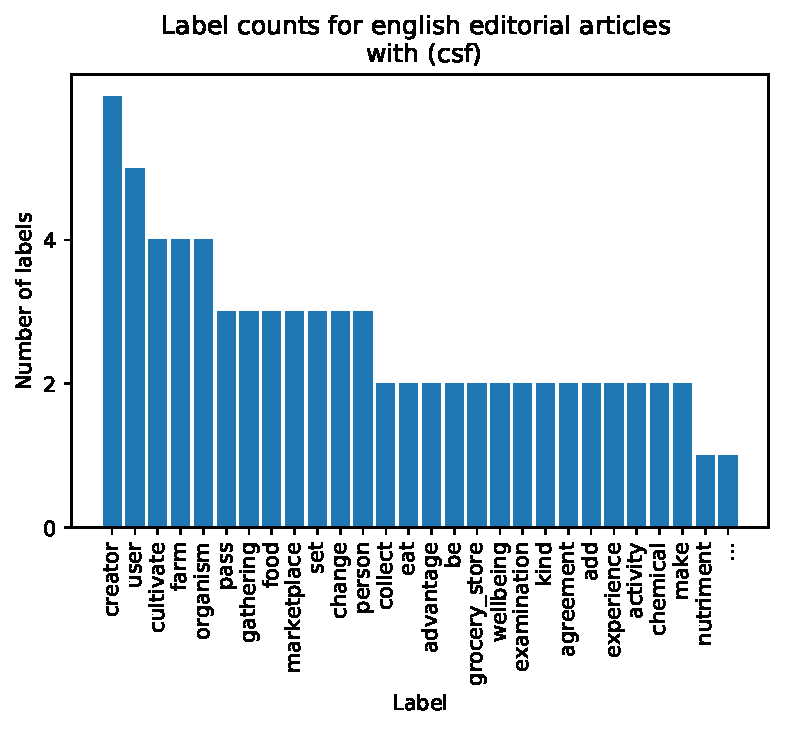
\includegraphics[width=7cm, height=7cm]{gfx/ATL_sim/with_scoring_pre.pdf}
	\end{minipage}
	\begin{minipage}[t]{0.5\textwidth}
		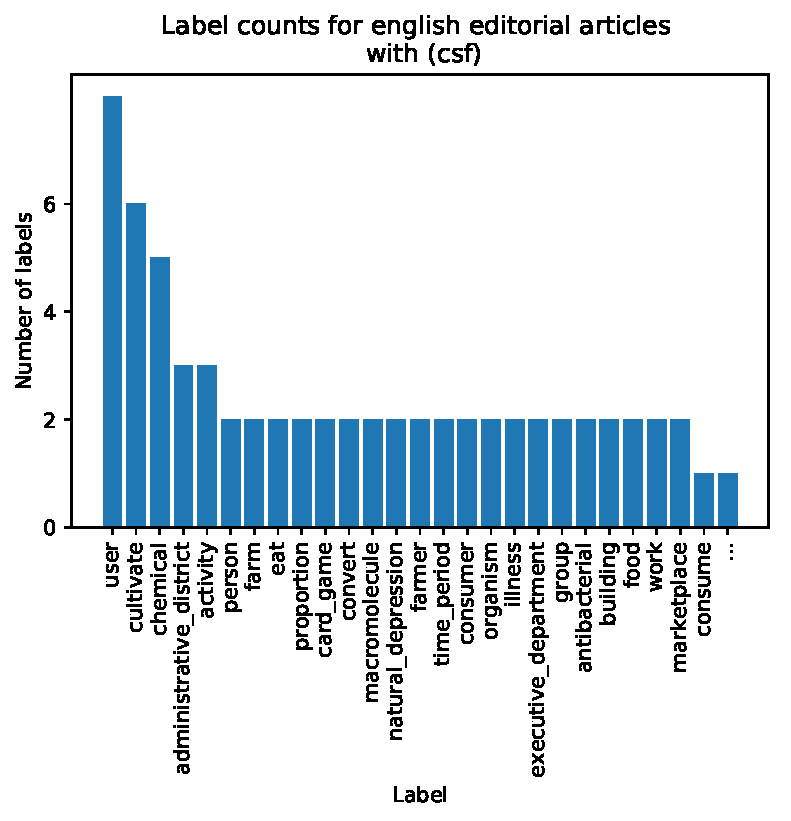
\includegraphics[width=7cm, height=7cm]{gfx/ATL_sim/with_scoring.pdf}
	\end{minipage}
	\caption{Label counts for topics from Generation 1 with \ac{csf}.}
	\label{extr_csf_count}
\end{figure}
%resume: 

Evaluated the intrinsic and extrinsic automatic topic labeling we can conclude, that the intrinsic approach generates meaningful and specific labels not really fitting to the topics and the extrinsic approach partially generates good results, which are comparable with the labels from the domain experts. Nevertheless, finding meaningful and high qualitative labels is not yet automatable. The knowledge and experience a human person has, can not be replaced by a machine.
%Based on our findings we can conclude that finding meaningful and high qualitative labels is not yet automatable. The knowledge and experience a human person has, can not be replaced by a machine.
%TODO comparison ja oder lieber weglassen?
%%%tabelle mit hannas
%\begin{table}
%	\begin{minipage}[t]{0.5\textwidth}
%		\begin{tabular}{c|ll}
%			&Topic 107 &\\
%			\hline
%			method & \multicolumn{2}{l} {\thead{waste, compost, use, scrap, material, \\landfill, ton, environmental, throw, gas}} \\
%			\hline
%			path & material 	& material  \\
%			ich  & abstraction	& physical entity\\
%			res  & material		& material\\
%			jsn  & abstraction	& material\\
%			lin  & material		& material\\
%			plg & waste	& abstraction\\
%			\ac{csf} & convent  & lowland\\
%			manual & \multicolumn{2}{l}{waste}	\\
%			&\\
%			%{topic 107}
%		\end{tabular}
%	\end{minipage}
%	\begin{minipage}[t]{0.5\textwidth}
%		\begin{tabular}{c|ll}
%			&Topic 23 &\\
%			\hline
%			&\multicolumn{2}{l} {\thead{grow, garden, plant, farm, vegetable, \\seed, year, tomato, produce, farming}} \\
%			\hline
%			&entity 	& produce  \\
%			&entity	& produce\\
%			&produce		& produce\\
%			&produce	& produce\\
%			&produce		& produce\\
%			&vegetable	& vegetable\\
%			&cultivate  & cultivate\\
%			&\multicolumn{2}{l}{homegrown food}	\\
%			&\\
%			%{topic 23}
%		\end{tabular}
%	\end{minipage}
%	\begin{minipage}[t]{0.5\textwidth}
%		\begin{tabular}{c|ll}
%			&Topic 64 &\\
%			\hline
%			method & \multicolumn{2}{l} {\thead{milk, raw, dairy, product, cheese,  cow\\health, drink, study, claim }} \\
%			\hline
%			path & abstraction 	& beverage  \\
%			ich  & abstraction	& produce\\
%			res  & dairy product		& beverage\\
%			jsn  & produce	& beverage\\
%			lin  & beverage		& beverage\\
%			plg & dairy product	& abstraction\\
%			\ac{csf} & nakedness  & farm\\
%			manual & \multicolumn{2}{l}{dairy product}	\\
%		\end{tabular}
%	\end{minipage}
%	%{topic 64}
%	\begin{minipage}[t]{0.5\textwidth}
%		\begin{tabular}{c|ll}
%			&Topic 74 &\\
%			\hline
%			&\multicolumn{2}{l} {\thead{meat, feed, beef, animal, grass, \\eat, raise, cow, buy, make}} \\
%			\hline
%			&entity 	& meat  \\
%			&entity	& abstraction\\
%			&matter		& meat\\
%			&food	& meat\\
%			&matter		& meat\\
%			&cattle	& physical entity\\
%			&cattle  & be\\
%			&\multicolumn{2}{l}{animal husbandry}	\\
%		\end{tabular}
%	\end{minipage}
%	%{topic 74}
%	\label{tab: labeled extrinsic and manually}
%	\caption[Labeled topics with extrinsic methods and manually]{Topics labeled manually and with extrinsic methods. Labels including preprocessing are in the third and fifth column.}
%\end{table}
%
%
%
%%%tabelle ohne hannah
%\begin{table}
%	\begin{minipage}[t]{0.5\textwidth}
%		\begin{tabular}{c|ll}
%			&Topic 19 &\\
%			\hline
%			method & \multicolumn{2}{l} {\thead{fish, salmon, choice , seafood, farm,\\farmed, catch, ocean, aquaculture, wild}} \\
%			\hline
%			path & physical entity 	& food  \\
%			ich  & physical entity	& food\\
%			res  & food		& food\\
%			jsn  & physical entity	& fish\\
%			lin  & location		& fish\\
%			plg & fish	& fish\\
%			\ac{csf} & food  & food\\
%			& \multicolumn{2}{l}{}	\\
%		\end{tabular}
%		%{topic 19}
%	\end{minipage}
%	\begin{minipage}[t]{0.5\textwidth}
%		\begin{tabular}{c|ll}
%			&Topic 27 &\\
%			\hline
%			& \multicolumn{2}{l} {\thead{fertilizer, soil, nutrient, plant, use, \\nitrogen, need, compost, hydroponic, water}} \\
%			\hline
%			& physical entity 	& physical entity  \\
%			& physical entity	& physical entity\\
%			& substance		& matter\\
%			& nutrient	& abstraction\\
%			& substance		& matter\\
%			& chemical	& chemical\\
%			& chemical  & substance\\
%			& \multicolumn{2}{l}{}	\\
%		\end{tabular}
%		%{topic 27}
%	\end{minipage}
%	\begin{minipage}[t]{0.5\textwidth}
%		\begin{tabular}{c|cc}
%			&Topic 122 &\\
%			\hline
%			method & \multicolumn{2}{l} {\thead{pesticide, chemical, glyphosate, toxic,\\use, spray, herbicide, weed, farmer, crop}} \\
%			\hline
%			path & chemical 	& chemical  \\
%			ich  & chemical	& chemical\\
%			res  & chemical		& chemical\\
%			jsn  & pesticide	& chemical\\
%			lin  & chemical		& chemical\\
%			plg & pesticide	& chemical\\
%			\ac{csf} & chemical  & chemical\\
%		\end{tabular}
%	\end{minipage}
%	%{topic 122}
%	\begin{minipage}[t]{0.5\textwidth}
%		\begin{tabular}{c|cc}
%			&Topic 100 &\\
%			\hline
%			& \multicolumn{2}{l} {\thead{child, baby, parent, kid, make, \\chemical, lead, home, mother, old}} \\
%			\hline
%			& child 	& child  \\
%			& child	& child\\
%			& relative	& child\\
%			& child	& child\\
%			& relative	& relative\\
%			& child	& person \\
%			& offspring   & offspring\\
%		\end{tabular}
%	\end{minipage}
%	%{topic 100}
%	\label{tab: labeled only extrinsic}
%	\caption[Labeled topics with extrinsic methods]{Labeled topics with extrinsic methods. Labels including preprocessing are in the third and fifth column.}
%\end{table}